\documentclass[border=5pt]{standalone}
\usepackage{tikz}
\usepackage{xcolor}
\usetikzlibrary{calc,shadows.blur}

% J6 - Green connector rod
\begin{document}
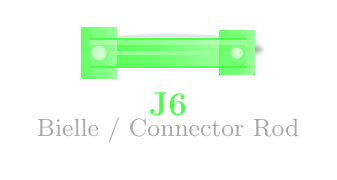
\begin{tikzpicture}

% Shadow
\fill[gray!20,blur shadow={shadow blur steps=5}] (1,0.12) ellipse (1.1 and 0.12);

% Rod body
\fill[left color=green!70, right color=green!30, middle color=green!55]
  (0.0,-0.18) rectangle (2.0,0.18);

% Left connector head (larger)
\fill[left color=green!60, right color=green!40]
  (-0.1,-0.32) rectangle (0.35,0.32);
\fill[green!50] (0.125,0) ellipse (0.11 and 0.32);

% Right connector head (smaller)
\fill[left color=green!60, right color=green!40]
  (1.65,-0.28) rectangle (2.1,0.28);
\fill[green!55] (1.875,0) ellipse (0.1 and 0.28);

% Bolt holes on heads
\fill[green!20] (0.125,0) circle (0.1);
\draw[green!50,thin] (0.125,0) circle (0.1);
\fill[green!20] (1.875,0) circle (0.08);
\draw[green!50,thin] (1.875,0) circle (0.08);

% Highlight
\fill[white,opacity=0.25] (0.0,0.1) rectangle (2.0,0.18);

% Center rib
\draw[green!40, line width=1.5pt] (0.35,0) -- (1.65,0);

% Outlines
\draw[green!70, line width=0.8pt] (0.0,-0.18)--(2.0,-0.18);
\draw[green!70, line width=0.8pt] (0.0,0.18)--(2.0,0.18);

% Label
\node[font=\bfseries\large, text=green!70] at (1.0,-0.65) {J6};
\node[font=\small, text=gray!70] at (1.0,-0.98) {Bielle / Connector Rod};

\end{tikzpicture}
\end{document}
